\chapter {Nutzung von Künstlicher Intelligenz auf eingebettete Systeme
}

\section{Anwendung, Beispiele zur erfolgreichen Implementierung von KI in eingebetteten 
Systemen}
\subsection{Spezielles Beispiel: Autonome Fahrzeuge}
Im Folgenden wird die Interaktion zwischen dem eingebetteten System und der KI am Beispiel eines autonomen Fahrzeugs näher erläutert.\\
Autonome Fahrzeuge, wie Autos und Busse, sind in der Lage, Hindernisse eigenständig zu erkennen und bei Bedarf anzuhalten. Diese Fähigkeit basiert auf einer Vielzahl von eingebetteten Systemen, die durch Künstliche Intelligenz  gesteuert werden. Wie in Abbildung \ref{fig:Kommu} dargestellt, verfügen autonome Fahrzeuge über eine komplexe Sensorik, darunter LIDAR, Radar, IMU (Inertiale Messeinheit), sowie Kameras und GPS-Antennen, die zusammenarbeiten, um Umgebungsdaten zu erfassen und zu analysieren.
\begin{figure}[h]
	\centering
	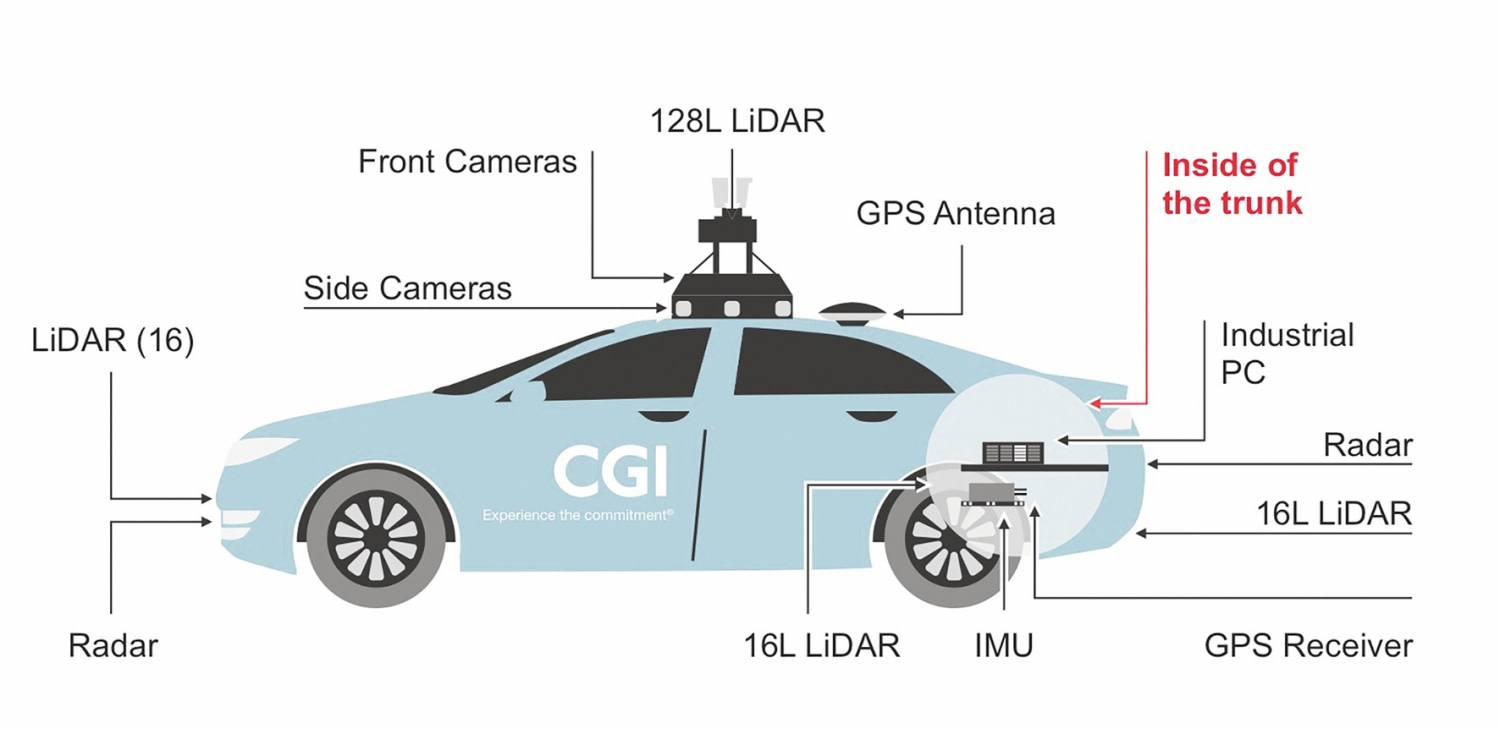
\includegraphics[width=0.9\textwidth]{img/Fahzeuge_GCI.jpg}
	\caption{Beispiel eines autonomen Fahrzeugs\textsuperscript{01}}
	\label{fig:Kommu}
\end{figure}
\footnotetext{\textsuperscript{1}Quelle: \url{https://www.hanser-automotive.de/a/fachartikel/besser-sein-als-der-mensch-211161}}

Die Abbildung \ref{fig:Kommu} zeigt die Architektur eines autonomen Fahrzeugs, bei dem mehrere Sensoren strategisch positioniert sind, um eine 360-Grad-Überwachung zu gewährleisten. Der LIDAR-Sensor spielt eine zentrale Rolle bei der Erstellung von präzisen 3D-Karten der Umgebung, während Radarsysteme die Erkennung von beweglichen Objekten wie anderen Fahrzeugen und Fußgängern unterstützen. Kameras sind unerlässlich für die visuelle Analyse von Verkehrszeichen, Straßenmarkierungen und Ampeln, was eine detaillierte Navigation ermöglicht. Die Kombination dieser Daten mit GPS-Positionierung sorgt für eine genaue Lokalisierung des Fahrzeugs auf digitalen Karten.\\
Durch diese Integration kann das Fahrzeug, wie in der Abbildung illustriert, Entscheidungen in Echtzeit treffen, zum Beispiel das Anhalten an Kreuzungen oder das Umfahren von Hindernissen. Hochleistungsrechner, wie sie in autonomen Fahrzeugen verwendet werden, ermöglichen die Verarbeitung der von den Sensoren gesammelten Daten und steuern das Fahrzeug entsprechend. Firmen wie Waymo und Tesla nutzen solche Architekturen, um die Sicherheit und Effizienz ihrer Systeme zu verbessern.\\
Die Abbildung verdeutlicht somit die wesentliche Rolle von eingebetteten KI-Systemen bei der Realisierung autonomer Fahrzeuge und dient als Beispiel für die erfolgreiche Integration von Sensorik, Aktorik und KI-gestützten Algorithmen.\\

\subsection{Weitere Beispiele von Anwendung von KI in eingebette Systeme}
Neben der Anwendung von KI in autonomen Fahrzeugen finden künstliche Intelligenz und eingebettete Systeme auch in zahlreichen anderen Bereichen vielfältige Einsatzmöglichkeiten. Ein Beispiel hierfür ist die "MindSphere"-Plattform von Siemens, eine offene IoT-Plattform, die in eingebetteten Systemen industrieller Anlagen integriert ist. Diese Plattform nutzt KI zur Analyse von Sensordaten von Maschinen, um potenzielle Ausfälle vorherzusagen und die Wartung zu optimieren. Durch den Einsatz von maschinellem Lernen kann das System kontinuierlich lernen und Anomalien in Produktionsprozessen frühzeitig erkennen, was die Effizienz und Zuverlässigkeit in der Industrie verbessert.\\
Auch im Bereich der Sicherheits- und Überwachungstechnik hat Hikvision Künstliche Intelligenz in seine eingebetteten Kamerasysteme integriert. Die abgebildete Kamera in Abbildung \ref{fig:hikvision} illustriert den Einsatz von KI-gestützter Überwachungstechnik, bei der fortschrittliche Bildverarbeitungsalgorithmen und maschinelles Lernen eine zentrale Rolle spielen. Die Systeme ermöglichen eine präzise Erkennung von Personen in Echtzeit sowie eine automatische Analyse von Verhaltensmustern. Dies erlaubt es, verdächtige Aktivitäten frühzeitig zu identifizieren und angemessen darauf zu reagieren.\\  

\begin{figure}[h]
	\centering
	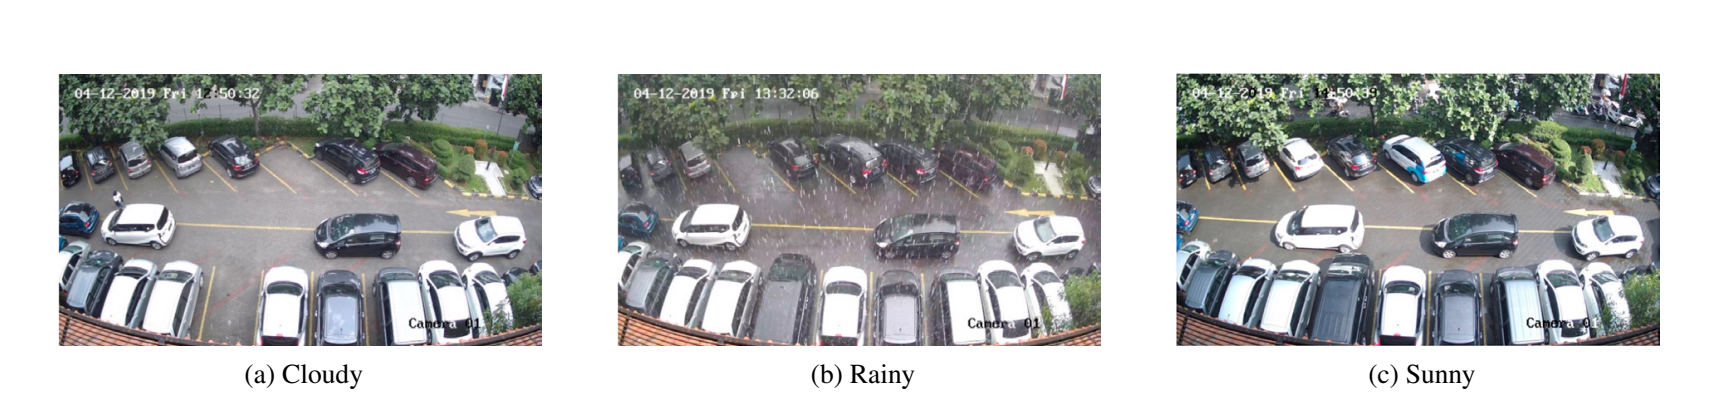
\includegraphics[width=0.9\textwidth]{img/hikvision_parking.png}
	\caption{Hikvision IP-Kamera zur Überwachung der Parkplatzbelegung \cite{Farley.2021}}
	\label{fig:hikvision}
\end{figure}  
Ein konkretes Anwendungsbeispiel für KI-gestützte Überwachungssysteme ist die automatische Erkennung von Parkraumbelegung. Die in Abbildung \ref{fig:hikvision} gezeigte Kamera nutzt Deep-Learning-Modelle wie AlexNet und mAlexNet, um in Echtzeit zwischen belegten und freien Parkplätzen zu unterscheiden. Die Forschungsergebnisse zeigen, dass diese Systeme eine Erkennungsgenauigkeit von bis zu 93,15 \% erreichen und eine Parkplatzanalyse innerhalb von 0,5 Sekunden pro Stellplatz durchführen können \cite{Farley.2021}.  

Durch den Einsatz dieser Technologie wird die Effizienz von Parkraummanagementsystemen erheblich gesteigert. Autofahrer können schneller freie Parkplätze finden, was nicht nur den Verkehrsfluss verbessert, sondern auch den Kraftstoffverbrauch und die Umweltbelastung reduziert. Die Integration von KI in solche Überwachungssysteme zeigt, wie maschinelles Lernen und eingebettete Systeme zur Optimierung urbaner Infrastrukturen beitragen können.\\  

Die Implementierung von Künstlicher Intelligenz in eingebettete Systeme eröffnet eine Vielzahl neuer Anwendungen, bringt jedoch auch Herausforderungen mit sich. Da eingebettete Systeme oft unter Echtzeitbedingungen operieren und mit begrenzten Rechenressourcen arbeiten, ist eine effiziente Implementierung von KI-Algorithmen entscheidend. Die Entwicklung solcher Systeme erfordert eine enge Verzahnung zwischen Hardware-Optimierung und Software-Design, um eine hohe Genauigkeit und geringe Latenzzeiten zu gewährleisten.  

\section{Vorteile und Herausforderungen der Integration von KI in eingebettete Systeme}

Eine der größten Chancen besteht in der Optimierung von Produktionsprozessen. Eingebettete KI-Systeme ermöglichen es Maschinen, selbstständig zu lernen und sich an veränderte Bedingungen anzupassen \cite{Gembaczka.2019}. In der Industrie können smarte Sensoren und Algorithmen genutzt werden, um Produktionsanlagen in Echtzeit zu überwachen, Maschinenausfälle vorherzusagen und Wartungen zu planen, bevor kritische Störungen auftreten. Dies minimiert teure Ausfallzeiten und maximiert die Effizienz. Darüber hinaus bietet die zunehmende Integration von KI im Internet der Dinge (IoT) erhebliche Vorteile. KI-gesteuerte eingebettete Systeme können die Kommunikation zwischen vernetzten Geräten verbessern, sodass Haushaltsgeräte, Fahrzeuge oder Fertigungsstraßen nahtlos miteinander interagieren können, um Muster zu erkennen und sich an Umgebungsbedingungen anzupassen \cite{Hamblen.2013}.

Ein weiteres Potenzial liegt in der Automobilindustrie, in der KI-gestützte, eingebettete Systeme bereits große Fortschritte erzielt haben, insbesondere bei der Entwicklung autonomer Fahrzeuge. Diese Systeme verarbeiten Sensordaten und Kamerabilder in Echtzeit, um präzise Entscheidungen über Fahrverhalten und Navigation zu treffen. Dadurch wird die Verkehrssicherheit erheblich verbessert und das Unfallrisiko verringert, was auch den Kraftstoffverbrauch optimiert und den Verkehrsfluss verbessert \cite{Koricanac.2021}. Ebenso haben KI-gesteuerte Systeme im Gesundheitswesen eine revolutionäre Wirkung. Geräte wie Herzschrittmacher oder tragbare Sensoren können durch KI intelligenter arbeiten, Gesundheitsdaten kontinuierlich überwachen und Unregelmäßigkeiten frühzeitig erkennen, was die Patientenversorgung verbessern könnte.

Trotz dieser bedeutenden Vorteile gibt es jedoch auch zahlreiche Herausforderungen bei der Integration von KI in eingebettete Systeme. Die begrenzte Rechenleistung und der Speicherplatz solcher Systeme stellen eine der größten Hürden dar. Im Gegensatz zu Cloud-basierten Anwendungen müssen eingebettete Systeme mit knappen Ressourcen auskommen, was die Implementierung komplexer KI-Algorithmen erschwert. Um diesem Problem zu begegnen, werden spezialisierte Hardwarebeschleuniger entwickelt, die es ermöglichen, leistungsstarke maschinelle Lernmodelle in kleinste Systeme zu integrieren \cite{Gembaczka.2019}. Eine weitere Herausforderung ist die Notwendigkeit der Echtzeitverarbeitung von Daten \cite{Mazzia.2020}. Eingebettete Systeme müssen oft sofort auf Veränderungen reagieren, was verlangt, dass KI-Algorithmen extrem effizient und zuverlässig arbeiten \cite{Mazzia.2020}.\\
In sicherheitskritischen Bereichen wie der Luftfahrt oder dem Automobilsektor können Verzögerungen oder Fehlentscheidungen schwerwiegende Folgen haben.
Zusätzlich ist der Datenschutz eine wesentliche Herausforderung. Da viele eingebettete KI-Systeme kontinuierlich Daten erfassen, müssen strenge Sicherheits- und Datenschutzmaßnahmen entwickelt werden, um die Privatsphäre der Nutzer zu schützen, besonders in Bereichen wie der medizinischen Überwachung oder engl. Smart Homes. Schließlich könnte die zunehmende Automatisierung durch KI auch soziale und wirtschaftliche Auswirkungen haben, insbesondere in der Industrie, wo automatisierte Fertigungsanlagen möglicherweise menschliche Arbeitskräfte ersetzen. Um diesen Herausforderungen zu begegnen, sind Weiterbildungs- und Umschulungsprogramme notwendig, damit Arbeitnehmer sich in der neuen KI-gesteuerten Arbeitswelt zurechtfinden können.
Insgesamt bieten eingebettete KI-Systeme transformative Möglichkeiten, sowohl in der Industrie als auch in Bereichen wie dem Gesundheitswesen und der Automobilindustrie. Dennoch erfordert die Integration dieser Technologien eine sorgfältige Berücksichtigung der technischen, ethischen und sozialen Herausforderungen. Nur durch eine ausgewogene Herangehensweise lässt sich das volle Potenzial der KI in eingebetteten Systemen ausschöpfen, während gleichzeitig Risiken minimiert werden.







